% !TEX root = DesignDocument.tex

\chapter{Design  and Implementation}
In this section, we describe the design details for each of the major components in our product. In this chapter, we will discuss the architecture and system design for our product, which includes the design selection, a diagram of the data flow in our product, communication and classes in each of the projects, and mock up screen-shots of all the GUI interfaces that our product has now or will have later. In addition, each of the major components of the product are described in more detail below.
 

\section{Architecture and System Design}
Part of our project is hosted in the cloud by Microsoft Azure. It is here that our database, web application, as well as our API are hosted. The web application is used to create the calendar data and store it in the database. This web application is responsible for the creation of accounts, whether it be a student, professor, or other faculty member.  Once logged in, the web app can be used to create events for a faculty or room calendar.  When the calendar is created, all the events can be viewed and modified on the main dashboard screen.\\


The web API can be used to get the needed data from the database and show the calendar on the tablet application.  The API has a number of calls to get data for the tablet app based on certain parameters.  There is a login endpoint which will give a token based on correct authentication input.  There are also a number of endpoints used to return a list of events based on certain criteria such as room or faculty names.\\

The tablet application uses these API calls and displays the data accordingly.  As mentioned above, it first uses a token endpoint where it sends the inputted user name and password in a body to the API.  The response given back determines if the user is authenticated or not.  If successful, the user can access all other API get event calls while using this authentication token.

  

\subsection{Design Selection}
A majority of our design for this project was directly affected by our decision on hardware.  Our hardware options were between an Android tablet or an ODroid based setup. The ODroid environment included many parts: an ODroid, a display, a camera, a wifi adapter, and a few other parts. As for the Android tablet, we needed to figure out the best tablet that fit our project needs. So after some deliberation, we went with a Samsung Galaxy Tab 8A for our hardware.  This tablet was about the same cost as an ODroid system.  We determined it would be better to focus this product on software that is able to be used on any Android device.  The potential few dollars we would save on an ODroid was not worth the setup time to configure the whole device.\\

The next decision to be made was whether to write our code in an exclusive Android environment and code the iOS applications later, or write the code using Xamarin forms for cross platfom development. We decided to save time in the future by writing it using Xamarin now. So the tablet application and the mobile application are being written using Xamarin forms.

Edit: Starting in the Spring semester of Senior Design, we are no longer using Xamarin forms for the tablet application of this project.  All developent will be done in Android Studio..........

 
\subsection{Data Structures and Algorithms}
This program follows the dataflow shown in Figure ~\ref{overallDataflow}. This is in a sense our algorithm.  The data will be created using a webportal where the information is stored in the database.  From here we will use the API to grab the needed data and display it on the tablet.  The API will have calls allowing us to grab data such as daily events, professor infomation, special messages, etc.\\

For example, a user can create an account or log in to the web application. Once authenticated, he or she can create an event on the calendar by clicking where the event is to be started, dragging the mouse to the end time of the event.  A box will then come up wich allows the user to edit the name of the event, and manually adjust the times.  Once the user saves this event, it is stored in the database.  We now need a way for this data to be sent to out tablet application.  This is where the API is used.\\ 

A user can then log into the tablet application (Which needs the API as well), and select the calendar that was just edited in the web application.  When the user syncs the calendar, the tablet application uses a API get call to retrieve all events which match the selected calendar.  The API will go to the database, find all events which match the calendar in the call, and return a list of calendar events.  The tablet application can then parse this response, and use the data to display the events.
 
\subsection{Data Flow}
Below is a diagram that shows the data flow for this project. Each of the components shown in the diagram are described in Figure ~\ref{overallDataflow} in greater detail. The figure shows how the database, web API, and the web application connect together and pass data back and forth.The figure also shows how this data is passed to and from the tablet application.
 
\begin{figure}[h!]
\centering
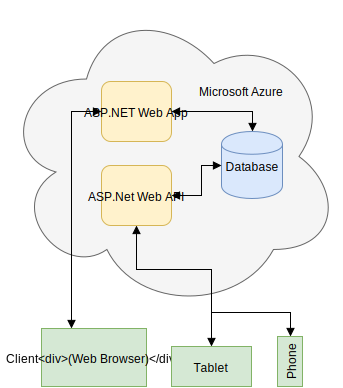
\includegraphics[scale=0.5]{DesignImages/OverallDataFlow.png}
\caption{Project Dataflow}
\label{overallDataflow}
\end{figure} 
 
\subsection{Communications}
One of the main communications in this project is between our RESTful API and the tablet application. A RESTful API uses HTTP requests to GET, POST, PUT, and DELETE. These requests return data in a JSON formatted string for the tablet to consume. The other communications in this project are the web app with the database and the web API and the database.\\

The HTTP client used for communication between the tablet application and the API is called Retrofit. It is a type safe HTTP REST client for Java. Retrofit provides a framework for interacting with API's and sending network requests with OKHTTP. There is also built in JSON parsing.  The JSON responses returned by the API calls can be parsed and filled into defined Java Objects.  
 
 
 
\subsection{Classes}
Here is a list of classes used by the web application and by the web API projects.
\begin{itemize}
\item Account Controller Class - Manages the accounts 
\item Calendar Controller Class - Manages the calendar events
\item Home Controller Class - Manages the main homepages
\item Calendar Event Repository Class - Implementation of the methods for calendar events
\item ICalendar Event Repository Class - Interface, lists methods for calendar events
\item University Context Class - Connects the models to the database
\item Account Binding Models Class - Used for handling accounts
\item Account View Models Class - Used for handling account views
\item Calendar Event Class - Model outline for the calendar events
\item Identity Models Class - Used for authenticating an identity
\item Instructor Class - Model outline for an instructor, inherits from person
\item Office Personnel Class - Model outline for an office personnel, inherits from person
\item Person Class - Model that contains and checks input for first and last name
\end{itemize}

\begin{figure}[h!]
\centering
\includegraphics[scale=0.35]{DesignImages/DoorPanesWebAppHome.PNG}
\caption{Web Application Website Homepage}
\label{webAppHomePage}
\end{figure} 

\begin{figure}[h!]
\centering
\includegraphics[scale=0.35]{DesignImages/DoorPanesWebAppLogin.PNG}
\caption{Web Application Login Page}
\label{webApplicationLoginPage}
\end{figure} 

\begin{figure}[h!]
\centering
\includegraphics[scale=0.4]{DesignImages/DoorPanesWebAppCal.PNG}
\caption{Web Application Calendar Controller}
\label{webApplicationCalView}
\end{figure} 
 
\subsection{GUI}
Figure \ref{webAppHomePage}, Figure \ref{webApplicationLoginPage}, and Figure \ref{webApplicationCalView} are the application's current GUI screenshots:


Figure \ref{fig:login}, Figure \ref{fig:firstview}, Figure \ref{fig:selection}, Figure \ref{fig:dashboard}, Figure \ref{fig:finallogin}, and Figure \ref{fig:navdrawer} are the wireframe mockups of the user interfaces of the tablet application.  Figure \ref{fig:ScreenArchitecture} in section \ref{ArchitectureSection} shows how all of these screens connect.
 
\begin{figure}
\centering
  \includegraphics[scale=0.4]{login.png}
  \caption{Login page}
  \label{fig:login}
\end{figure}


\begin{figure}
\centering
  \includegraphics[scale=0.4]{firstview.png}
  \caption{Preview Page}
  \label{fig:firstview}
\end{figure}

\begin{figure}
\centering
  \includegraphics[scale=0.4]{selection_final.png}
  \caption{Preview Page}
  \label{fig:selection}
\end{figure}

\begin{figure}
\centering
  \includegraphics[scale=0.4]{dashboard.png}
  \caption{Dashboard view}
  \label{fig:dashboard}
\end{figure}

\begin{figure}
\centering
  \includegraphics[scale=0.4]{dashboard_final.png}
  \caption{Login page}
  \label{fig:finallogin}
\end{figure}

\begin{figure}
\centering
  \includegraphics[scale=0.4]{navigationdrawer.png}
  \caption{Dashboard view with navigation drawer expanded}
  \label{fig:navdrawer}
\end{figure}

\begin{figure}
\centering
  \includegraphics[scale=0.4]{contact.png}
  \caption{Contact Professor page}
  \label{fig:contactprof}
\end{figure}

\pagebreak
\section{Major Component \#1 - ASP.NET Web API}

\subsection{Technologies  Used}
\begin{itemize}
\item Microsoft Azure
\item Microsoft Visual Studio
\item Web Browsers
\item ASP.NET Razor markup
\end{itemize} 

\subsection{Component  Overview}
\begin{itemize}
\item Endpoints
\begin{itemize}
\item Login
\item Get Calendar Events
\item Get Calendar Events By Date
\item Get Calendar Events By Professor
\item Get Calendar Events By Room
\item Get A Calendar Event
\item Get A Instructor
\item Get Office Personnel
\item Add/Update/Delete Calendar Event
\item Add/Update/Delete Instructor
\item Add/Update/Delete Office Personnel
\item Add/Update/Delete Student
\end{itemize}
\item Models
\begin{itemize}
\item Instructor
\item Office Personnel
\item Student
\item Person
\item Calendar Event
\end{itemize}
\item Controllers
\begin{itemize}
\item Instructor
\item Office Personnel
\item Student
\item Calendar Event
\end{itemize}
\item Repositories
\begin{itemize}
\item Calendar Events Interface
\item Calendar Events
\item Instructor Interface
\item Instructor
\item Office Personnel Interface
\item Office Personnel 
\end{itemize}
\end{itemize}

\subsection{Phase Overview}
\begin{itemize}
\item Gathered User Stories
\item Researched and Designed
\item Process of Application Development
\end{itemize}

\pagebreak
\subsection{Dataflow Diagram}
\begin{figure}[tbh]
\begin{center}
\includegraphics[scale=0.5,width=0.75\textwidth]{MVC5.png}
\caption{Web API Dataflow Diagram}
\end{center}
\label{APIMVC}
\end{figure}

\section{Major Component \#2 - ASP.NET Web App}

% This section was written by Andrew Fagrey

\subsection{Technologies  Used}
This section describes the various technologies used for the ASP.NET web application. Since the web application is hosted in Microsoft Azure, Azure handles most of the backend for keeping the web application up and running. The server that the web application is running on and the storage for the web application are all handled by Microsoft. In addition, Azure handles the publicly accessible URL for the web application. Here's a full list of the technologies we are currently using to support the web application:

\begin{itemize}
\item Microsoft ASP.NET Web App Framework
\item Microsoft MVC App Framework
\item Microsoft Azure Cloud Services
\item Microsoft Azure Database
\end{itemize}


\subsection{Component  Overview}
This section is a description of the various software components used in the web application. The web application is divided up into three main sections software-wise: the models, the views, and the controllers.\\

The web application models are classes that provide an abstraction and a representation of the data that is passed around in the web application. For example, the web application has a model for a calendar event, which contains fields pertaining to calendar details, like an event title, a start and end time, and an event owner.\\

The web application views contain the code that generates the HTML web pages that are viewed in a web browser. The view files are C\#-based files that make use of a Microsoft feature called Razor. Basically, Razor allows the C\# code to be intertwined with HTML code. This allows us to, for example, use C\# to generate an HTML list element without actually coding all the list tags ourselves.\\

The web application controllers are the classes that are used by the ASP.NET web application routing system to determine what code is run based on the URL given in a web browser. Each method inside the controller class corresponds to a different endpoint in the web application. As we develop the web application, we will have controllers for managing the various calender views, controllers for office personnel, and controllers for classrooms.\\

Below is a current list of the components that the web app either has or will have:


\begin{itemize}
\item A website homepage showcasing the product 
\item A login page accessible by a web browser
\item Calendar dashboard for viewing, creating, and editing calendar events
\item An open source calendar framework for displaying JavaScript-based events on the calendar framework
\item A website URL, which is currently www.doorpaneswebapp.azurewebsites.net
\item A convenient way to quickly cancel a set of events for a specific day
\end{itemize}


\subsection{Phase Overview}
This section describes the various development phases for the web application. This section is currently being updated as the development of the web application continues. Below is a list of development phases we went through as we developed the web application:

\begin{enumerate}
\item Gathered user stories for the web application
\item Built a test web application
\item Started to modify the web application to reflect the DoorPanes project
\item Published the web application on Microsoft Azure Cloud to start testing how it worked and what it looked like
\item Began developing and integrating calendar models and the open source calendar framework.
\item Currently working on expanding the model and controller list in conjunction with the web API.
\end{enumerate}


\subsection{Dataflow Diagram}
This section contains a dataflow diagram for the web application. The dataflow diagram shown in Figure ~\ref{webAppDataflow} shows how the data moves inside the web application.\\\\

\begin{figure}[h!]
\centering
\includegraphics[scale=1.0]{DesignImages/webAppDataflow.png}
\caption{Web Application Dataflow Diagram. Image by Microsoft.}
\label{webAppDataflow}
\end{figure}

% CITE IMAGE
% https://docs.microsoft.com/en-us/aspnet/core/tutorials/first-web-api

\section{Major Component \#3 - Android Tablet Application}

\subsection{Technologies  Used}
To develop the tablet application for this project, Android Studio version 2.2.2 will be used. All testing for this project will be used on a Samsung Galaxy Tab 8A tablet running Android version 6.0 (Marshmallow) The target level for the execution of this application will be Android 6.0, API level 23. All testing done in Android will use Espresso testing framework.\\

In summary, here are the technologies used:

\begin{itemize}
\item Android Studio Version 2.2.2
\item Android SDK - target API level 23
\item Samsung Galaxy Tab 8A
\item Espresso Testing Framework
\end{itemize}



\subsection{Component  Overview}
The main goal of the tablet application is to display a schedule for a given classroom or professor. After logged in, a user can cycle through given schedules and look at different views: daily, weekly, and monthly.  There will also be a contact feature that will allow the user to send a message or email to a professor. \\

Here are the components that the tablet application will have when finished:

\begin{itemize}
\item A login page on application startup
\item A calendar preview/selection page
\item Dashboard view for viewing the chosen calendar
\end{itemize}

\subsection{Phase Overview}


Below is a list of the development phases of the tablet application:

\begin{itemize}
\item Gathered user stories
\item Set up Android environment
\item Created the login view
\item Created calendar select view
\item Created dashboard view
\item Create navigation menu 
\item Use API calls to get calendar information 
\item Create contact forms (pending)
\item Create different calendar views (pending)
\end{itemize} 


\subsection{ Architecture  Diagram}
\label{ArchitectureSection}
The architecture design for the tablet application is shown in Figure ~\ref{fig:Architecture}. The program will start on a login screen when open. If login is successful, a preview page will be shown. From this preview page, the user can select a schedule to be shown from a list of available schedules from the account. Once selected, the program goes to the dashboard view
\begin{figure}[h!]
  \includegraphics[width=\linewidth]{graph.png}
  \caption{Architecture Diagram}
  \label{fig:ScreenArchitecture}

\end{figure}
